\chapter{Future work}

This chapter briefly describes the required steps for the sensor to be able to fly on-board PW-Sat2.

\section{Qualification model}
    Firstly, the sensor will be implemented on a PC-104 factor board, together with all final components and procedures. The model shown is taken from the design process (figure \ref{PLD_BOARD}).

    \begin{figure}[H]
        \centering
        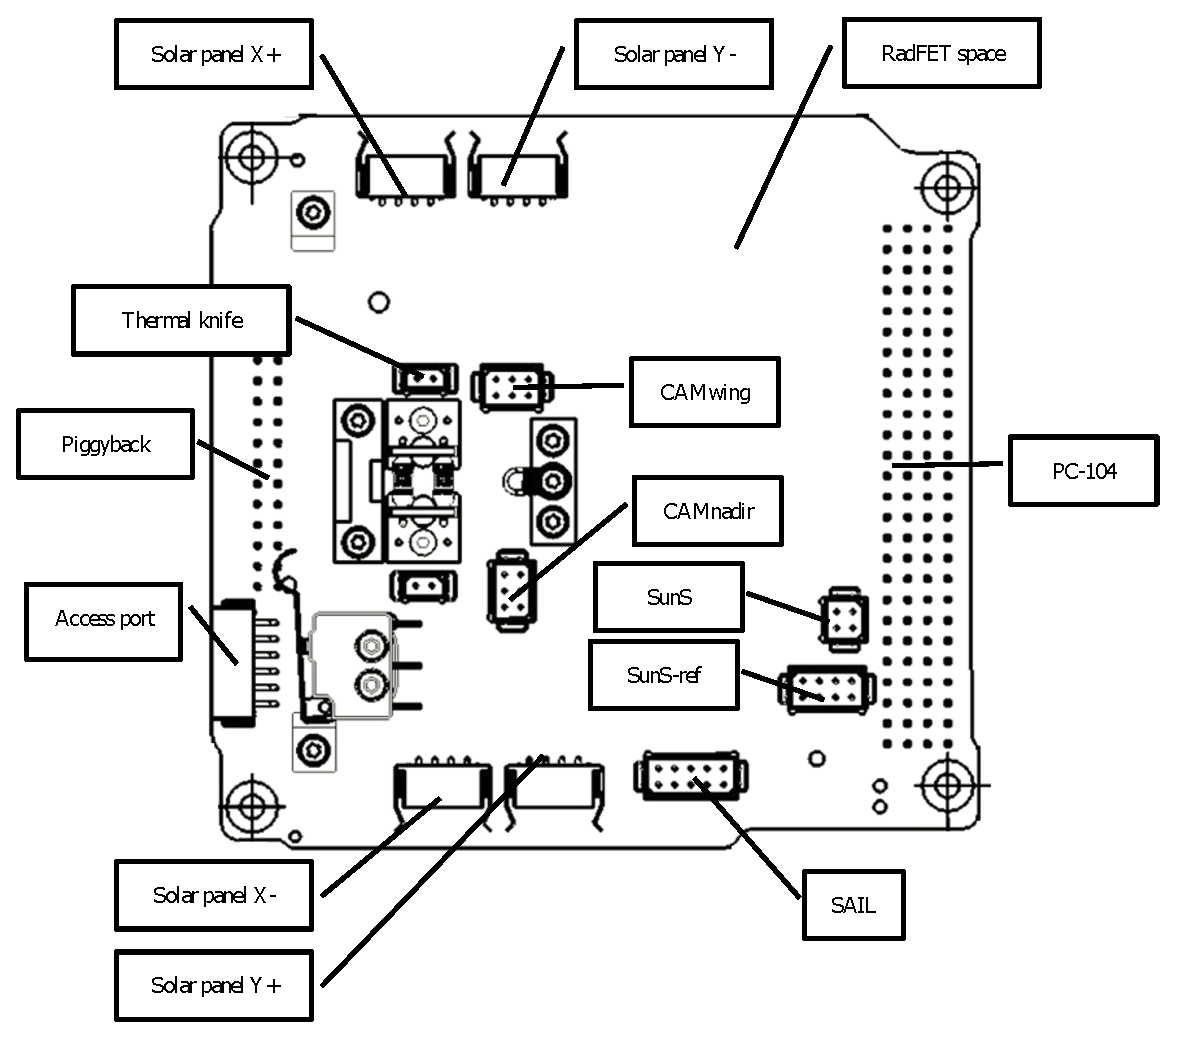
\includegraphics[width=0.7\paperwidth]{img/08/PC104pldBoard.eps}
        \caption{PLD board with connector and space designed for RadFET}
        \label{PLD_BOARD}
    \end{figure}


    On this model all software tests (on flat-sat) will be carried out, as well as the final confirmation of design (thermal, radiation and time-stability tests). This board will qualify sensor design and software for flight use.

\section{Flight model}
    In the end, a final flight version of the PCB will be manufactured. In principle, it should be identical to the Qualification Model, but the handling procedures will be much more strict. Additionally, on the flight model, only thermal calibration will be made, without further stress-testing. During integration, the final version of the sensor on PC104-board will be placed on the electronics stack inside PW-Sat2.
